\documentclass[tikz,border=10pt]{standalone}
\begin{document}
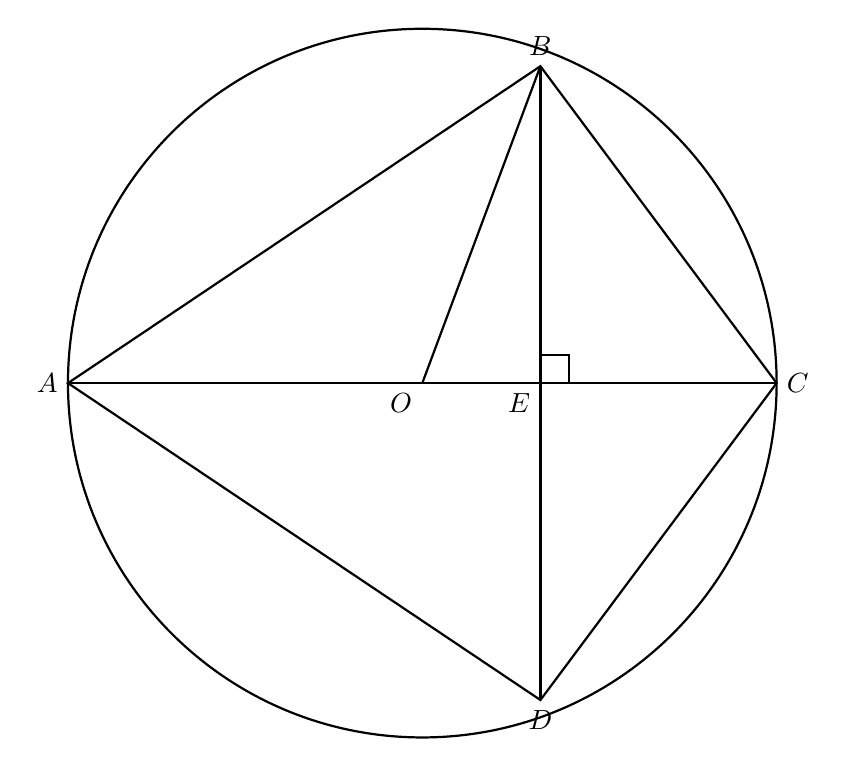
\begin{tikzpicture}[scale=3,thick]
\coordinate (O) at (0,0);
\coordinate (A) at (-1.5,0);
\coordinate (C) at (1.5,0);
\coordinate (E) at (0.5,0);
\coordinate (B) at (0.5,1.3416);
\coordinate (D) at (0.5,-1.3416);
\draw (O) circle (1.5);
\draw (A) -- (C);
\draw (B) -- (D);
\draw (A) -- (B) -- (C) -- (D) -- cycle;
\draw (O) -- (B);
\draw (0.5,0.12) -- (0.62,0.12) -- (0.62,0) -- (0.5,0);
\node[below left] at (O) {$O$};
\node[left] at (A) {$A$};
\node[above] at (B) {$B$};
\node[right] at (C) {$C$};
\node[below] at (D) {$D$};
\node[below left] at (E) {$E$};
\end{tikzpicture}
\end{document}
